\title{The Adaptive Multi-scale Simulation Infrastructure - Design and Application}
\author{W.R. Tobin, V.W.L. Chan, M.S. Shephard}
\date{\today}
\documentclass[11pt]{siamltex1213}
\bibliographystyle{siam}

\usepackage{amsfonts}
\usepackage{graphicx}
\usepackage{listings}
\usepackage{mathtools}
\DeclarePairedDelimiter\ceil{\lceil}{\rceil}
\DeclarePairedDelimiter\floor{\lfloor}{\rfloor}

\lstset{basicstyle=\small, 
        stringstyle=\ttfamily, 
        frame=top, frame=bottom,
        captionpos=t}

\begin{document}
\maketitle

\begin{abstract}
\end{abstract}

\section{Note}\label{note}
This article predominantly discusses multi-scale simulations - wherein two or more separate physical scales are involved in the simulation - the discussion is equally applicable to multi-model simulations - wherein two or more numerical or physical models operating on the same domain (possibly with differing discretizations) are involved in the simulation - as well as to simulations which are both.

\section{Introduction and Motivation}\label{introduction}
\label{single_scale_simulations}
Most physical models and implementations using numerical methods operate at a single scale characteristic to the problem. The scale at which the preponderance of attributes governing the underlying physics being modelled are measured and the resolution of the numerical solution is considered acceptable for the desired accuracy of the simulation.

\label{multi_scale_simulations}
Introducing multi-scale influences on the scale of interest in a simulation can occur in several places during the development of a simulation. Most fundamentally, the influence can be incorporated during the mathematical development of the physical model itself. In this case the multi-scale features are incorporated into the numerical implementation automatically, as a result of their presence in the mathematical model. 

Multi-scale influences can also be incorporated in a numerical sense, combining established physical models operating at different scales referencing and effecting shared physical fields and values \cite{shenoy97} \cite{weinan2003heterogenous}. Numerically multi-scale simulations associate many numerical implementations of single-scale physical models and cause them to interact by passing key physical terms between scales. This operation, referred to as scale-coupling, involves up-/down-scaling operations to account for differences in scale dimensionality (and possibly dimensionalizing terms computed in a non-dimensional domain).

In order for a numerically multi-scale approach to be effective the domain associated with the scale of interest (or engineering scale) must be sufficiently large that conducting the entire simulation with terms and granularity orders of magnitude removed would make the simulation computationally intractable. Thus some computationally reasonable subset of the engineering scale is assigned tertiary scale(s) to simulate. The precise choice of location of the tertiary simulations is largely dependent on the specific numerical algorithms used to implement the engineering scale simulation.

Often the subset of the domain associated with the tertiary scales are areas of the engineering domain where the impact of the tertiary scales has the most impact on the engineering scale simulation, in order to leverage the most utility from the multi-scale approach.

Numerical multi-scale simulations fall broadly into two categories. In the concurrent multi-scale paradigm, all scales are computed simultaneously and the required inter-scale coupling values are provided just-in-time \cite{zeng2010concurrent}. In the sequential multi-scale paradigm, tertiary scales compute parameters which are converted to quantities of utility to a primary scale. Each scale (though not necessarily each scale-task, representing an individual operation or simulation occurring in a scale) must be processed sequentially \cite{garcia2008sequential} and may be blocked on the completion of the previous scale. This multi-scale model maps intuitively to phased parallel communication models found in the commonly used bulk synchronous parallel abstraction \cite{valiant1990bridging}. 

\subsection{Adaptive Multi-scale Simulation Infrastructure}\label{amsi}
The Adaptive Multi-scale Simulation Infrastructure (amsi) is a set of libraries and tools developed at the Scientific Computation Research Center (SCOREC) at Rensselaer Polytechnic Institute. Amsi is designed to support the implementation and execution of dynamic numerically multi-scale simulations on massively-parallel HPC machines. Currently amsi provides interfaces for describing and managing the execution of individual scales in a multi-scale simulation, for defining, managing and enacting the scale-coupling communication required by such simulations, and for planning and enacting scale-sensitive load balancing operations on individual scales in a multi-scale system.

The interfaces provided by the amsi libraries are intended to facilitate the coupling of functional (possibly legacy) simulation codes already in usage for single-scale problems, in order to avoid development overhead associated with casting a simulation into a set of framework-specific components. The currently implemented interfaces are physics-agnostic, operating only on computational quantities with no model of a term's relation to the mathematical derivation of the multi-scale interaction. Incorporation of meta-information and services targeted toward specific multi-scale physical couplings represents a desirable extension of the amsi libraries, constituting a rich area of future work.

Amsi operates by maintaining a set of minimal simulation metadata in order to model various quantities of interest during simulation execution. A decentralized approach toward control is taken; dynamic control decisions are made and implemented at runtime during collective operations. In order to avoid the introduction of unnecessary parallel barriers into the code, amsi control decisions are only made during operations which are already collective over the set of processes effected by a given control decision.

Frameworks and runtime systems have been developed which are intended for the development of specific multi-scale problems \cite{parker2006component} \cite{chopard2011framework} \cite{} and these frameworks have in some cases been expanded to facilitate the implementation of additional multi-scale problems \cite{berzins2010uintah}.

These systems suffer from the requirement that an application developer must cast the problem of interest into a set of predefined components (interfaces, tasks, etc.) or specify the problem through a high-level modelling language in order to take full advantage the services provided by the framework. Leveraging a component-based design is valuable from a software engineering perspective, but also introduces new complexities involved in defining the set of components and how they interoperate in the framework, shifting some complexity up the abstraction hierarchy. The core features of amsi used for multi-scale simulation management and communication are provided with no requirements of adherence to a specific component definition.

Typically simulation flow control is determined solely by the runtime system. A framework may also limit specific features of the numerical implementation to those provided by the framework. This includes domain discretization models and associated adaptive processes -- structured and unstructured meshing and associated refinement algorithms, particle-in-cell methods, etc. -- convergence algorithms for both the minimization of the relevant residuals (Newton-Raphson, etc.) as well as iterative solution of the resulting linear system (KSP, GMRES, ILU, etc.). 

Amsi supplies several numerical components consisting of an adaptive finite element system, linear algebraic solver, and nonlinear convergence operators available as both simple C++ class interface definitions, as well as implementations of these interfaces built on top of other software supplied by SCOREC \cite{core} for finite element analysis operations as well as the PETSc linear algebraic solver \cite{petsc-web-page} \cite{petsc-user-ref} \cite{petsc-efficient}. Usage of the supplied numerical components is not required to make use of the multi-scale meta-modeling, communication, dynamic instantiation, and scale-sensitive load balancing facilities supplied by amsi.

Implementing required numerical operations inside an existing framework is of course possible, though it may prove an additional -- undesirable overhead for an application programmer interested only in utilizing the multi-scale framework to implement a simulation, rather than implementing the various numerical operations often optimized in widely available packages and libraries.

\section{Methods}

\label{amsi_scales}
A configuration file is supplied during command invocation containing the initial configuration of the process sets and their assignment to individual scales, as well as declaring the coupling between scales in the simulation. The declaration of a scale and the initialization of the process set associated with the scale are considered a single atomic operation in the current implementation. 

Process sets are mathematical sets of MPI ranks implemented so as to take advantage of any mathematical conveniences to minimize explicit storage whenever possible. Process sets are required to be non-overlapping in order for amsi control mechanisms to operate correctly. Ongoing developments are targeted at removing this requirement to allow a richer set of dynamic control options and increase overall utilization in the case of coupled scales blocking on one another. 

Scales are an abstraction grouping a set of standalone scale-tasks operating on a single scale, the set may be as minimal as a single scale-task as in the case of a primary scale with many contributing tertiary scales. The set may also contain many individual scale-tasks which all operate within a single scale, such as when a primary scale-task has an associated tertiary scale which constitutes many individual simulations, as in the biotissue example case discussed in section \ref{biotissue}. Precisely what defines a scale-task is left up to the user, the intent is for each scale-task to represent a standalone single-scale simulation incorporated into the multi-scale system.

A scale coupling is a relation denoting that scale-coupling communication will take place between two scales at some point during the simulation. Declaration of a coupling relation between two scales is required for communicating scales, as the coupling declaration during simulation initialization is used to instantiate data structures specific to scale-coupling operations. This limits memory overhead by not allocating space for unneeded coupling operations. This coupling relationship is asymmetric, thus if scale A is related to scale B (ie. A produces terms required for B to operate), scale B is not implicitly related to scale A, though this may be separately declared.

A simple configuration file can be seen in listing \ref{amsi_config_file} which declares the existence of two scales, macro and micro\_fo, and tells the amsi intialization procedures to assign them process sets containig 64 and 8128 processes, respectively (for a total of $2^{13}$ processes). The file also specifies the scale-coupling relations, with macro coupled to micro and micro coupled to macro. Note that the order of specification is not relevant to the operation of amsi.
%
\begin{lstlisting}[caption={amsi\_config file},label=amsi_config_file]
  macro 64
  micro_fo 8128
  #
  macro micro_fo
  micro_fo macro_fo
\end{lstlisting}
%

Dynamically creating the required configuration file as part of a shell script invoking the simulation is straightforward. Alternative specification mechanisms such as ratio specification (equivalently percentage specification) are being considered for future implementation to prevent the possibility of misallocating processes (the user not specifying assignment for all processes available to the simulation, or attempting to overallocate processes).

The assignment of processes to a process set is static, and processes cannot be reassigned during a simulation. Additionally the assignment of a scale to a process set is static as well. The application programmer may provide capabilities for scale-tasks to be dynamically created and destroyed at runtime, amsi provides functions to inform coupled scales of such dynamic modifications. Since scale-tasks are an abstraction the amsi systems cannot provide direct operations on scale-tasks, but provide mechanisms for the application to inform amsi of such operations when they occur.

Additionally, scale-tasks associated with specific subsets of a process set (either a single process or several processes) may be migrated in part or in whole. Migrating a scale-task in part amounts to using load balancing facilities on the associated processes to redistribute all data scale-task from a scale-task to a subset of the previously associated processes, allowing the freed processes to be assigned data from other scale-tasks. Migrating a scale task in whole constitutes using load balancing operations on the process set associated with the entire scale to move all pertinent data between subset of the managed process set. Amsi provides operations to enact load-balancing operations from plans such as those generated by Zoltan algorithms.  In the current implementation these operations are collective on the process set associated with the managed scale.

While the primary scale (the scale associated with producing the solution for the overall simulation) is often thought of as controlling the tertiary scales in terms of dynamic instantiation, this is not assumed in the amsi implementation. Any scale is capable of informing the process set associated with a coupled scale of the addition or deletion of individual scale-tasks. At present it is dependent on the developer to implement the capability of a scale to accept additional scale-tasks.

\label{amsi_communication}
Scale-coupling communication is guided by data distributions and communication patterns. A data distribution is a representation of individual units of scale-coupling data distributed across a single scale-task. The format of the coupling data is arbitrary (so long as it can be serialized and provided for use by MPI communication primitives). A data distribution represents the smallest unit of data important to the scale-coupling communication, which is necessarily distinct for various multi-scale use cases. 

Scale-linking quantities are dynamically registered with the amsi system using a data distribution defined on a scale by the scale-tasks operating at that scale. Production of a communication pattern is required prior to executing a scale-coupling communication, and the pattern must be reconciled (synchronized across the coupling relationship) prior to being used to guide a coupling communication operation (and when the communication pattern is altered by the scale providing the coupling data). Several simple communication pattern production algorithms are provided by amsi, but these are relatively trivial due to the nature of scale-coupling communications and the general nature of the amsi libraries. Hooks are provided for users to implement algorithms for the construction of communication patterns tailored to the specifics of their problem. 

A communication pattern based on the relationship of scale $A$ coupled to scale $B$ is thought of most simply as a matrix $C \in \mathbb{N}^{|A|\times|B|}$ (where $|X|$ is the cardinality of the process set currently assigned to scale X). The implementation of the communication pattern uses a sparse format in order to reduce the memory impact as the simulation scales. The quantity $C_{ij}$ represents the quantity of scale-coupling terms (of arbitrary type) to be sent from process $i$ in the process set assigned to $A$ to process $j$ in the process set assigned to $B$.

All communication and planning operations in the amsi libraries use an implicit local numbering for data distribution terms, the index associated with the term in a local serialized buffer. Usage only of implicit ordering was decided upon in order to reduce the memory impact as the simulation scales, as any meta-data which scales with the simulation will necessarily pose a memory issue once scaling hits some threshold.

At present an application developer must implement up-/down-scaling operations required for their particular multi-scale use case, hooks will be provided in future releases to automate application of such operations during scale-coupling. The current implementation includes blocking versions of the scale-coupling communication operations. Asynchronous versions have been designed but are not currently implemented due to lack of immediate need in the primary amsi use case.

\subsection{Soft Tissue Simulation}\label{biotissue}
The Biotissue code is a multi-scale simulation of soft organic tissues, consisting of an engineering-scale simulation using the finite element method, and a micro-scale quasistatics force-balance simulation. The Cauchy Momentum Balance Equation for a body in static equilibrium is used as the governing equation for the macro-scale simulation. 
%
\begin{align}
\nabla \cdot \pmb{\sigma} =& \; 0 \text{ in } \Omega \label{momentum_balance} \nonumber \\
\pmb{\sigma} \cdot \pmb{n} =& \; \pmb{t} \text{ on } \partial \Omega \nonumber
\end{align}
%
Specific quantities needed to compute the elemental tangent stiffness matrices and force vectors are instead supplied by the micro-scale force-balance simulations, which occur at each numerical integration point in the engineering-scale mesh \ref{biotissue_hierarchy}. 
%
\begin{figure}
  \begin{center}
    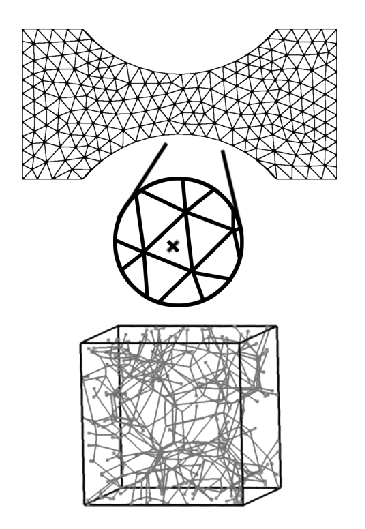
\includegraphics[height=2in]{biotissue_visual_hierarchy.eps}
  \end{center}
  \caption{\small biotissue multi-scale problem}
  \label{biotissue_hierarchy}
\end{figure}
%

The incremental displacements (deltas generated by the previous Newton-Raphson iteration) on each engineering-scale finite element node are used to distort the a dimensionless representative volume element (RVE) through a dimensionalized abstraction of the RVE embedded in the engineering domain and an associated displacement mapping term $\frac{d\mathbf{RVE}}{d\mathbf{FE}}$, the first order relation between the incremental displacement of an RVE with respect to the displacement of the associated mesh element. This results in each micro-scale node being displaced. Each RVE is a dimensionless unit cube containing a connected collagen fiber network, for the present results the fibers are implemented as truss elements and their distribution is generated using Delauney triangulation, resulting in a high coordination number at each node and consequently a numerically stable fiber network. The micro-scale boundary condition necessitates that the force exerted by each fiber network node located on the boundary of the RVE be zero. The micro-scale global Jacobian is formulated along with the force vector, wherein the boundary condition is enforced by setting specific rows of the force vector associated with boundary nodes to zero. 

Another Newton-Raphson iterative process occurs at micro-scale to converge to the set of displacements resulting in force equilibrium for all the fibers within the fiber network constituting the RVE. After a micro-scale simulation converges to a solution, the Jacobian and force vector are then evaluated again at the solution position, the force exerted along the boundary of the RVE is summed for each of the principal and shear components of a stress tensor, which is then dimensionalized and sent back to the engineering-scale for use in the elemental tangent stiffness matrix formulation. More detail into the derivation of this multi-scale system can be found in \cite{stylianopoulos2008thesis} \cite{agoram2001coupled} \cite{stylianopoulos2007multiscale} . Discussion of the dimensionalization of the dimensionless force terms produced by each fiber network can be found in \cite{stylianopoulos2007volume} \cite{chandran2007deterministic}.

The simulation two nested Newton-Raphson operations occurring; during each macro-scale Newton iteration every micro-scale RVE must undergo a full Newton-Raphson convergence process.

\section{Results and Discussion}\label{results}
The biotissue simulation was run on the AMOS BG/Q machine housed at the CCI facilities. Both strong and weak scaling studies were conducted up to an eighth of the total machine core count, or 16384 cores. The ratio of macro-scale to micro-scale assigned processes was held at 1:127, and the total core count was kept as an integer power of 2 in order for the SLURM job scheduler to submit the jobs to the compute nodes in a timely manner. The precise calculation used to determine macro and micro process counts is given by 
%
\begin{lstlisting}[language=Bash,caption={process assignment calculation}]
  NP=$(( $NUM_MACRO * 128))
  NUM_MICRO=$(( $NP - $NUM_MACRO))
\end{lstlisting}
\label{macro micro ratio}
%

Separate timings were taken for various sections of the simulation code, isolating the micro-scale computation, macro-scale linear system assembly and calculation of elemental linear systems, and macro-scale linear system solution. In addition, the time for spent in the amsi subroutines for communication was also measured. Thus the behavior of each section of the code is independently evaluated in our scaling study, as well as the overall execution time.

%
\begin{figure}
  \begin{center}
    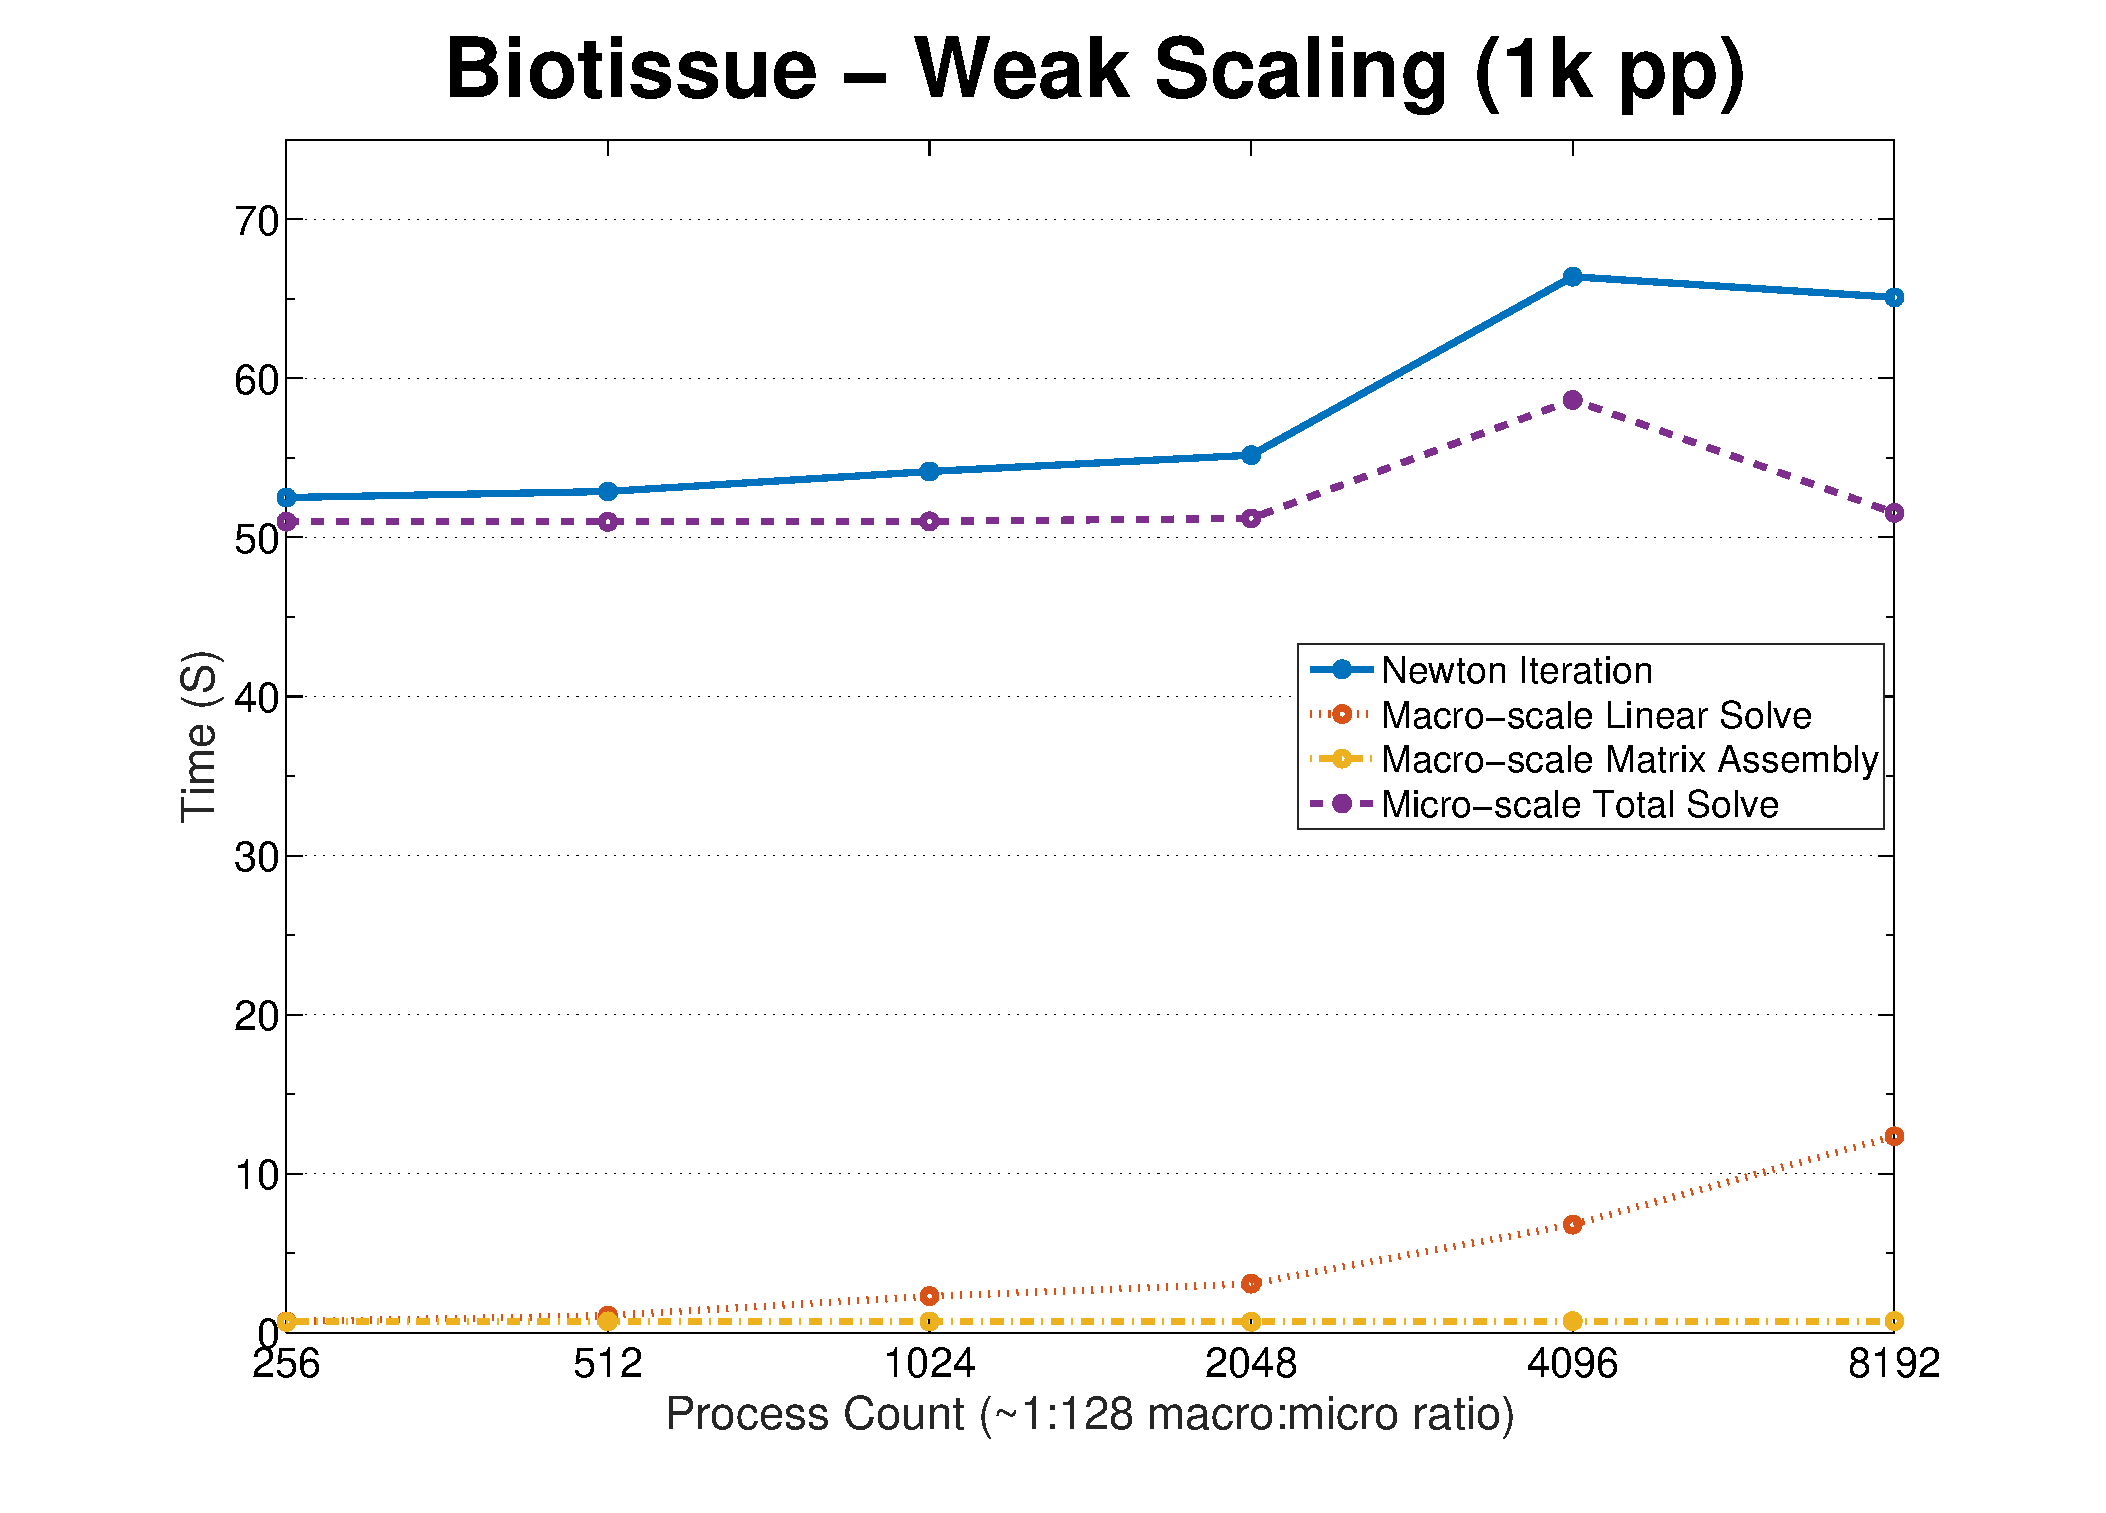
\includegraphics[height=2in]{ws_phil.eps}
  \end{center}
  \caption{\small weak scaling}
  \label{weak scaling}
\end{figure}
%
Keeping the work per process approximately constant (1k elements per macro-scale process, with the 1:127 macro-micro ratio as specified in listing \ref{macro micro ratio}) it can be seen that the time to compute every RVE in the system stays relatively consistent, while the time to solve the macro-scale linear system increases, causing a modest increase in the overall time per macro-scale Newton iteration.

%
\begin{figure}
  \begin{center}
    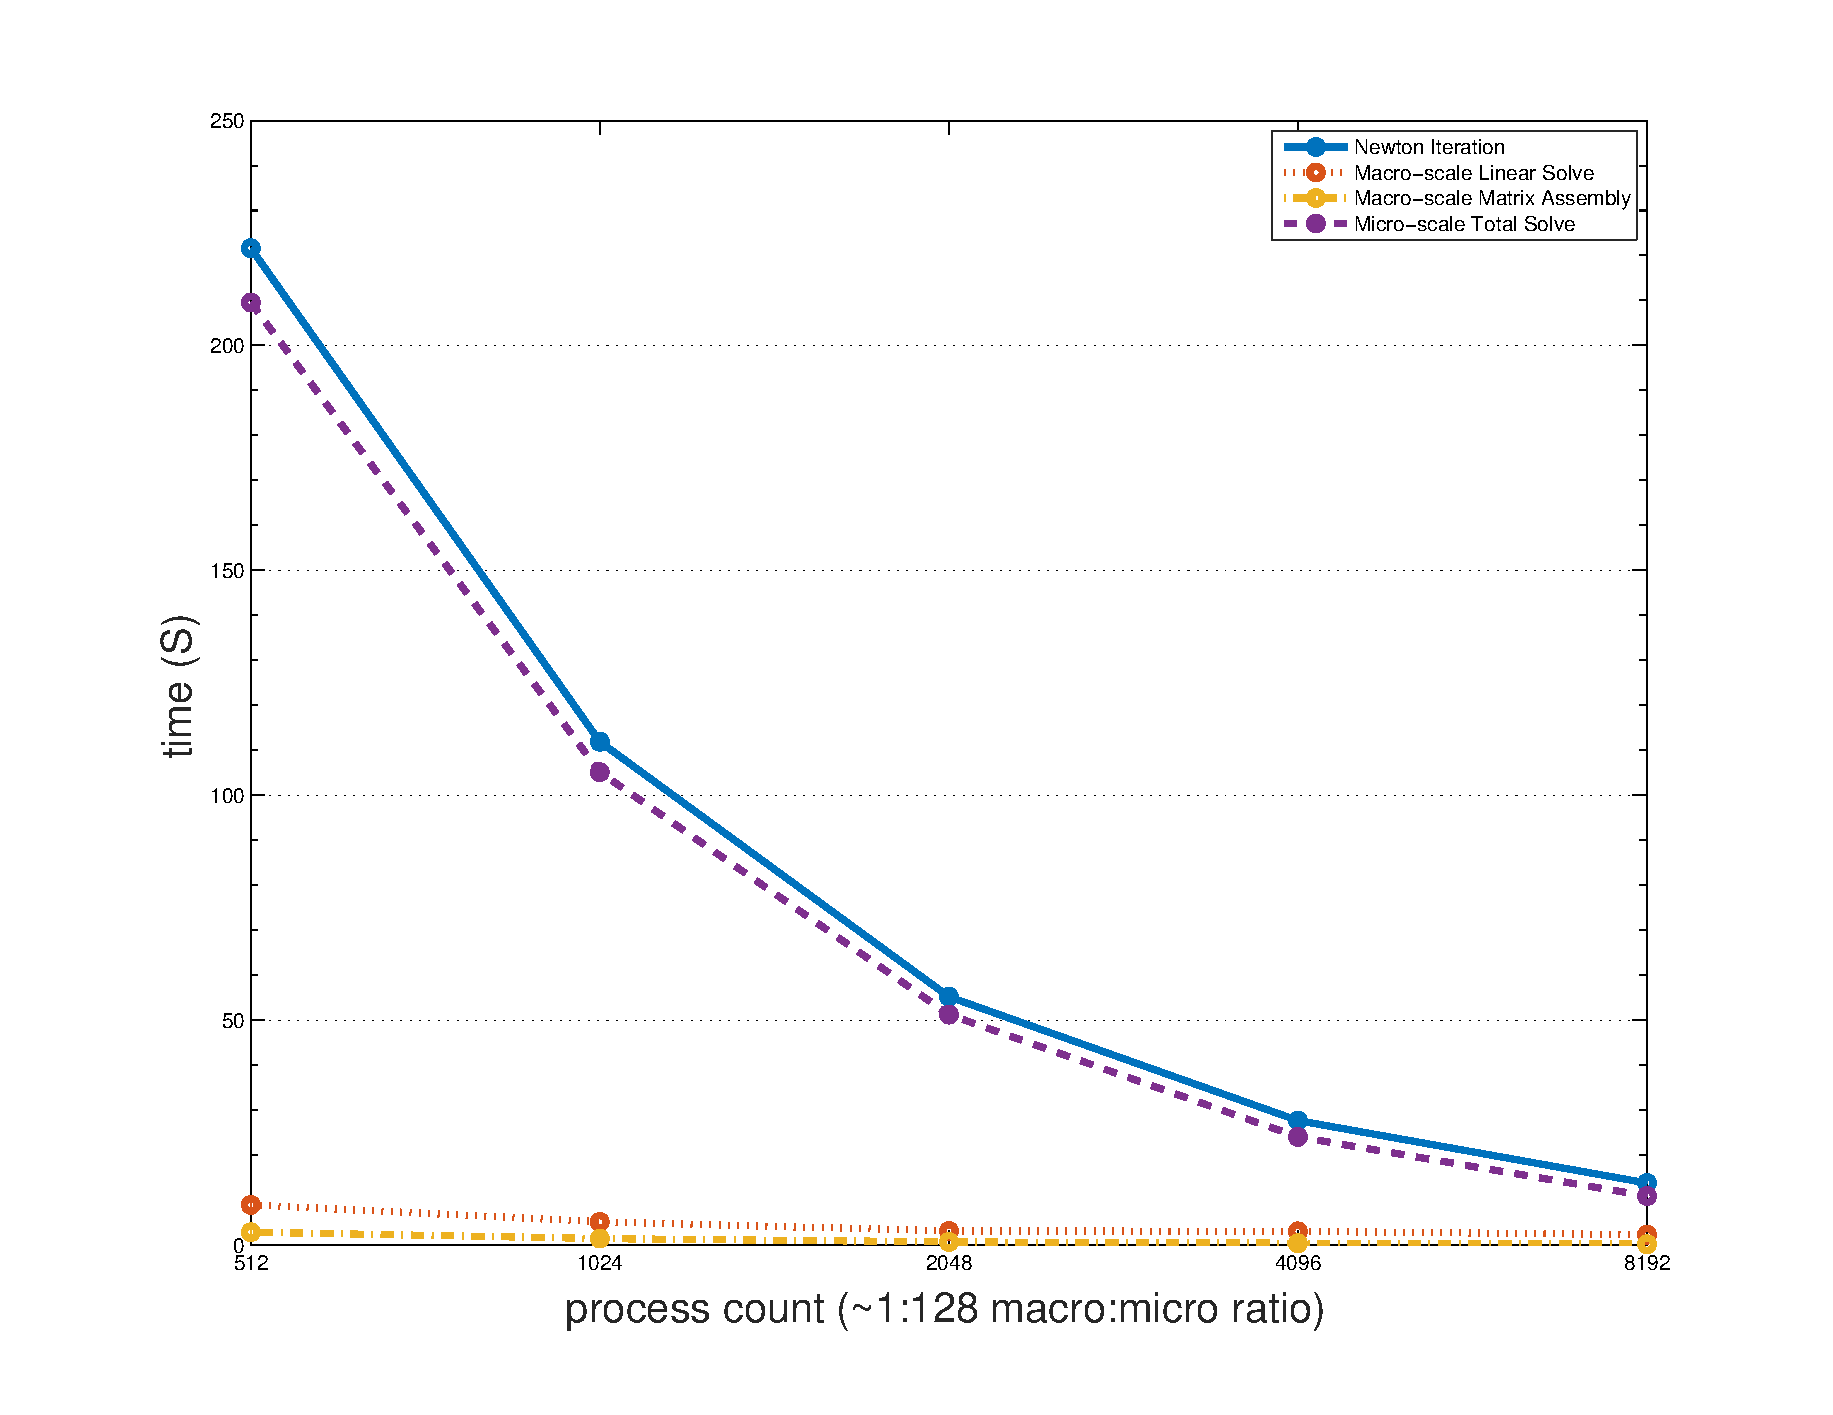
\includegraphics[height=2in]{ss_phil.eps}
  \end{center}
  \caption{\small strong scaling}
  \label{strong scaling}
\end{figure}
%
As the problem size is held constant with respect to the number of individual elements in the engineering scale domain discretization the simulation displays near optimal convergence to the macro-scale solve time alone, which is also reducing in time cost. The limiting factor in the speedup of the overall simulation is the potential speedup of the macro-scale simulation rather than the micro-scale simulation with fiber-only RVEs. As indicated in the weak scaling results this is related primarily to the macro-scale linear solve communication time increasing. At present an incomplete LU factorization is used to solve the linear system formulated at macro-scale each Newton iteraion (using PETSc configured with the superLU\_dist solver \cite{li05superlu} \cite{lishao10superluilu} \cite{lidemmel03superludist} ). Using instead an iterative solution method to reach a desired level of accuracy may result in stronger scaling at macro-scale, but as yet this approach has been unneeded due to the preponderance of time spent computing micro-scale results in use cases.

Many problems of interest will possess finite elements numbered in the tens to hundreds of millions of degrees of freedom, such that a suitable partitioning of the mesh to cores on the machine in terms of elements per partition (and directly the macro-scale time-to-solution) may require a substantial fraction of the total cores on the machine for macro-scale to execute in reasonable time. Amsi provides services for dynamically adding and removing individual scale-tasks to a specific scale, which can be utilized to limit RVE usage to only those locations in the multi-scale mesh most influential on the overall evolution of the simulation.

Amsi-specific results of some sort...?

Could include utilization/idle time metrics, but those are far more relevant to the load balancing paper...

\section{Conclusions and Future Work}\label{future_work}

The Adaptive Multi-scale Simulation Infrastructure provides a valuable set of tools to facilitate the implementation and execution of multi-scale simulations without imposing restrictions on the application developer. Usage of the core operations of the amsi libraries does not require adherence to a specific set of interfaces nor usage of an abstract modeling language, which complicate inclusion of legacy components into multi-scale simulations.

Scale-sensitive load-balancing operations have been developed for the biotissue multi-scale test problem. Unfortunately the problem does not exhibit load persistence in the current parallel execution space task discretization, so an alternative parallel discretization such as overdecomposition with work-stealing to enforce more local balancing operations and occasional global balancing operations is being explored.

Development of libraries concerned with higher levels of abstraction of the multi-scale problem will also be valuable in easing the development of new multi-scale simulations from the perspective of the application programmer. High level abstractions such as the Scale Separation Map in \cite{chopard2011framework} could provide mechanisms to provide initial configuration information to the amsi system during the initialization phase, as well as assist in the implementation of (or usage of existing library-provided) up-/down-scaling operations.

An RVE simulation taking into account inter-fibril matrix material has been developed \cite{lake2012mechanics} \cite{zhang2013cross} \cite{zhang2013coupled}. This alternative RVE will be incorporated into the multi-scale model as an alternative to the fiber-only RVE, to be used in areas of the macro-scale domain determined to be most critical to the overall evolution of the global system, or where error accumulation through model inaccuracy is to be minimized. As this fiber-matrix RVE represents a more significant source of computational complexity, it is independently parallelized -- in contrast to the fiber-only RVE -- and will represent a compelling use case for the parallel execution space discretization and scale-coupling communication management capabilities of the amsi libraries.
\bibliography{citations}

\end{document}
